\begin{frame}{debuggers / emulators}
    \begin{itemize}
    \item major way to analyzing software --- run it!
    \vspace{.5cm}
    \item possibly using debugger to analyze memory/registers/etc.
    \item possibly in restricted environment
        \begin{itemize}
        \item either limit access to system calls, \textit{or}
        \item run on virtual (okay-to-lose) hardware
        \end{itemize}
    \end{itemize}
\end{frame}

\begin{frame}{selected debugger features (1)}
    \begin{itemize}
    \item watchpoint (GDB/LLDB \texttt{watch})
        \begin{itemize}
        \item breakpoint triggered by variable/expression changing
        \end{itemize}
    \item breakpoints on system calls (GDB \texttt{catch syscall \ldots})
    \item searching memory for strings (GDB \texttt{find}, LLDB \texttt{memory find})
    \end{itemize}
\end{frame}

\begin{frame}{selected debugger fetures (2)}
    \begin{itemize}
    \item saving `core' files (GDB \texttt{generate-core-file NAME})
        \begin{itemize}
        \item full copy of program's memory, can reload in debugger later
        \end{itemize}
    \item copying memory to/from file (GDB \texttt{dump}/\texttt{append}/\texttt{restore}; LLDB \texttt{memory read}/\texttt{write})
    \item attaching to programs / remote debugging
    \item forcing jump to address/return from function (GDB \texttt{jump}/\texttt{return})
    \end{itemize}
\end{frame}

\begin{frame}{reverse debugging?}
    \begin{itemize}
    \item old idea: `reverse debugging'
    \item in addition to \texttt{step}/\texttt{continue}, \\
        debugger could have \texttt{reverse-step}/\texttt{reverse-continue}
    \item typically implemented by recording `trace' of execution
    \vspace{.5cm}
    \item some implementations (with varyingly middling performance
        \begin{itemize}
        \item \url{https://rr-project.org} for x86-64 Linux (needs sysadmin to set some things)
        \item QEMU for full virtual machines (not just one program)
        \item built-in to GDB, but not maintained/possibly broken with modern systems
        \end{itemize}
    \end{itemize}
\end{frame}

\begin{frame}{Ghidra debugger integration}
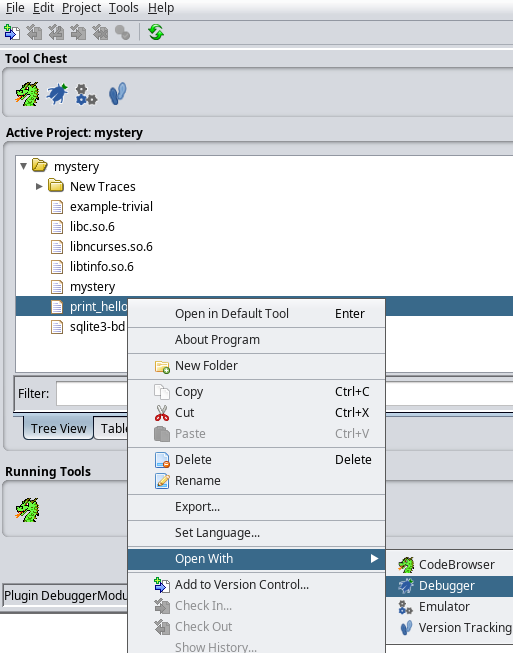
\includegraphics[width=0.35\textwidth]{../re-tools/ghidra-open-debugger.png}
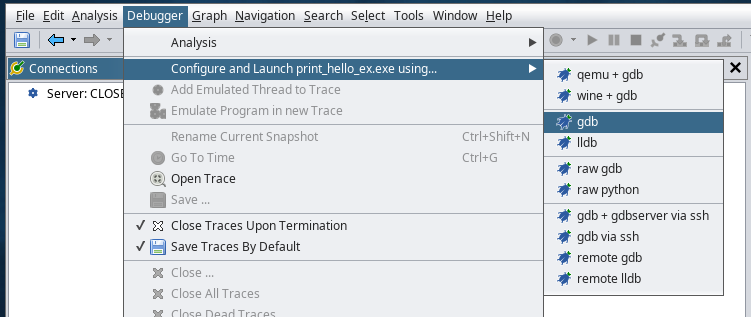
\includegraphics[width=0.55\textwidth]{../re-tools/ghidra-open-debugger2.png}
\end{frame}

\begin{frame}{aside: Ghidra debugger installation}
    \begin{itemize}
    \item relies on GDB python support + some python packages installed
    \item see installation docs
    \end{itemize}
\end{frame}

\begin{frame}{Ghidra traces}
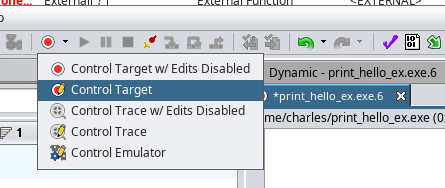
\includegraphics[width=0.3\textwidth]{../re-tools/ghidra-control-target.png}
    \begin{itemize}
    \item Ghidra --- debugging session creates a `trace'
        \begin{itemize}
        \item can be saved to look at later
        \end{itemize}
    \item creates a list of `snapshots' for every time debugger stopped
        \begin{itemize}
        \item snapshots are \textit{incomplete}
        \item need to force read of memory/etc. to have info included in snapshot
        \end{itemize}
    \item can switch between `Control Target' and `Control Trace' modes
        \begin{itemize}
        \item Control Trace --- go back to old snapshots, examine state
        \item Control Target --- control live program in debugger
        \end{itemize}
    \end{itemize}
\end{frame}

\begin{frame}{Ghidra dynamic view}
\begin{tikzpicture}
\node[inner sep=0mm,anchor=north west] (graphic) at (0, 0) {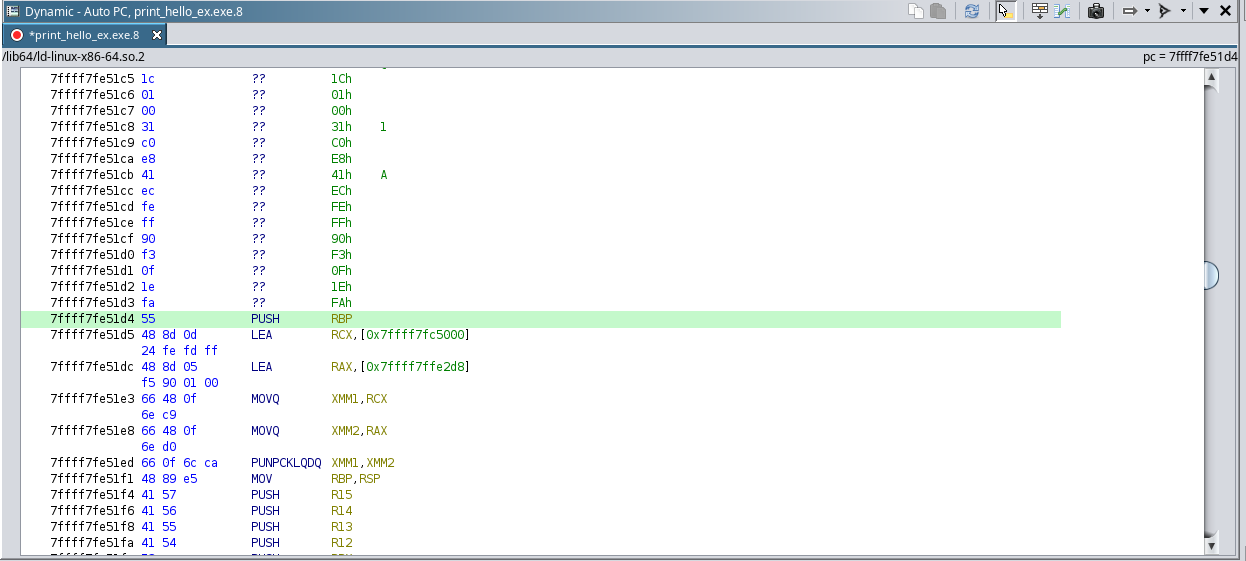
\includegraphics[width=13cm]{../re-tools/ghidra-dynamic}};
%\path[overlay,draw,help lines] (0, 0) grid (14, -8);
\begin{visibleenv}<2>
    \draw[red,thick] (.5, -3.2) rectangle (5, -5.8);
    \node[text=red,anchor=west,align=left] at (5, -5) {
        partial disassembly \\
        (starting from program counter)
    };
    \draw[blue,thick] (.5, -0.8) rectangle (5, -3.2);
    \node[text=blue,anchor=west] at (5, -2) {
        not disassembled by default
    };
\end{visibleenv}
\begin{visibleenv}<3>
    \draw[overlay,violet,thick] (10, 0) rectangle (10.3, -0.2);
    \node[overlay,text=violet,font=\small,anchor=east,align=right] at (10.1, -0.2) {
        reread selected memory
    };
    \draw[overlay,green!60!black,thick] (11.7, 0) rectangle (12.1, -0.2);
    \node[xshift=-1cm,overlay,text=green!60!black,font=\small,anchor=south,align=left] at (11.9, -0.0) {
        select where in \\
        memory to view
    };
\end{visibleenv}
\begin{visibleenv}<4>
    \draw[overlay,red,thick] (11, 0) rectangle (11.3, -0.2);
    \node[overlay,text=red,font=\small,anchor=east,align=right] at (11.3, -0.2) {
        compare memory at different times
    };
\end{visibleenv}
\end{tikzpicture}
\end{frame}

\begin{frame}{Ghidra snapshots/saved traces:}
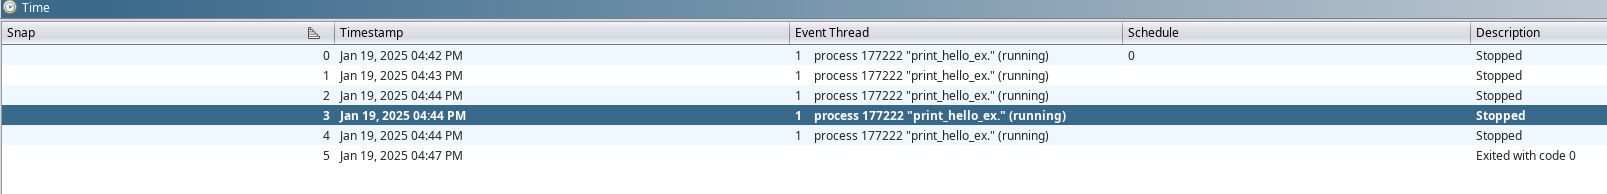
\includegraphics[width=\textwidth]{../re-tools/ghidra-time-trace}
\begin{itemize}
\item automatic partial snapshots whenever pausing debugger
\item can force read of range of memory to make snapshot contain memory image
\end{itemize}
\end{frame}
